% =====================================================================
%  Project-status presentation (Beamer, single-file)
%  What we have built and validated so far — the measurement half (Gate 1).
%  Build:  report/build.sh report/presentation   (Tectonic + Ghostscript-normalise)
% =====================================================================
\documentclass[aspectratio=169,11pt]{beamer}
\usetheme{default}
\setbeamertemplate{navigation symbols}{}
\setbeamertemplate{footline}[frame number]
\setbeamertemplate{itemize items}[circle]

\usepackage{amsmath,amssymb}
\usepackage{booktabs}
\usepackage{tikz}
\usetikzlibrary{positioning,arrows.meta,calc}
\usepackage{pgfplots}
\pgfplotsset{compat=1.18}

% --- self-contained palette (matches the proposal deck) ---
\definecolor{navy}{RGB}{30,64,124}
\definecolor{forest}{RGB}{34,120,60}
\definecolor{burnt}{RGB}{214,104,26}
\definecolor{plum}{RGB}{140,55,135}
\setbeamercolor{structure}{fg=navy}
\setbeamercolor{frametitle}{fg=navy}
\setbeamerfont{frametitle}{series=\bfseries}

\newcommand{\frozen}[1]{{\color{navy}\textbf{#1}}}
\newcommand{\ck}{{\color{forest}$\checkmark$}}
\newcommand{\done}{\ck}

\title[Project status]{Predicting the Zero-Shot Transfer of a Promptable Video Tracker}
\subtitle{Project status --- the measurement half, built and \emph{validated} (Gate\,1)}
\author{Kostiantyn Boiar}
\institute{MSc Dissertation \,\textbullet\, University of Glasgow\\[2pt]
\small Supervisor: Dr Marwa Mahmoud}
\date{\today}

\begin{document}

% ---------------------------------------------------------------- title
\begin{frame}[plain]
  \titlepage
\end{frame}

% ------------------------------------------------------------ the goal
\begin{frame}{The goal, in one sentence}
  \begin{block}{}
    \centering\large
    Given a \textbf{new animal} in a \textbf{new place}, predict how well SAM\,3 will track it ---
    \emph{before we run it} --- and explain \textbf{why}.
  \end{block}
  \vspace{0.6em}
  \begin{itemize}
    \item Separately for \textbf{finding} the animal (\texttt{pDetA}) and \textbf{following} it (\texttt{pAssA}).
    \item We are \emph{not} trying to make the tracker score higher --- we predict its \textbf{reliability}.
    \item Why it matters: conservation teams point these models at new species/regions constantly, and
          today \textbf{nobody can say in advance} whether to trust them.
  \end{itemize}
\end{frame}

% ------------------------------------------------------------ what SAM 3 is
\begin{frame}{What we measure: a promptable tracker, split in two}
  \centering
  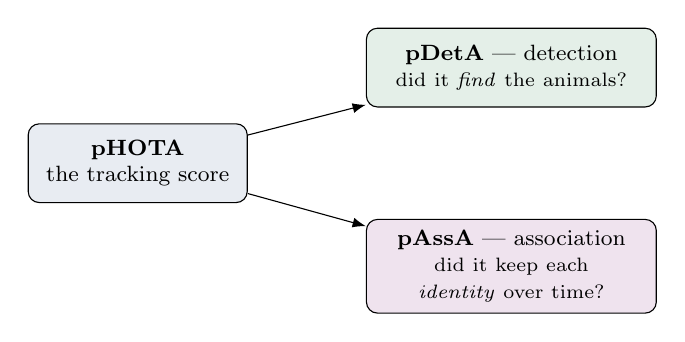
\begin{tikzpicture}[>=Latex,
    box/.style={draw,rounded corners,align=center,font=\footnotesize,inner sep=4pt,minimum height=1cm}]
    \node[box,fill=navy!10,text width=2.5cm] (h) {\textbf{pHOTA}\\the tracking score};
    \node[box,fill=forest!12,text width=3.4cm,above right=0.2cm and 1.5cm of h] (d)
        {\textbf{pDetA} --- detection\\\scriptsize did it \emph{find} the animals?};
    \node[box,fill=plum!14,text width=3.4cm,below right=0.2cm and 1.5cm of h] (a)
        {\textbf{pAssA} --- association\\\scriptsize did it keep each \emph{identity} over time?};
    \draw[->] (h) -- (d); \draw[->] (h) -- (a);
  \end{tikzpicture}
  \vspace{0.6em}
  \begin{itemize}\footnotesize
    \item \textbf{SAM\,3} is \emph{promptable}: type ``\texttt{impala}'' and it finds and follows every
          matching animal across a video --- with \textbf{no training on that species} (zero-shot).
    \item We analyse \textbf{finding} and \textbf{following} as two separate numbers --- that split is the
          intellectual core of the project.
  \end{itemize}
\end{frame}

% ------------------------------------------------------------ the data
\begin{frame}{The data --- SA-FARI}
  \begin{itemize}
    \item Thousands of short \textbf{camera-trap videos} of wild animals, every frame hand-outlined.
    \item \textbf{99 species} with a full tree-of-life $\cdot$ \textbf{741 locations} on 4 continents
          $\cdot$ a decade of footage (2014--2024).
    \item Keeps \textbf{hard negatives} --- a query for an absent animal, where a good model returns
          nothing (drives the false-positive check).
    \item Gated outlines from Hugging Face $+$ public frames from Google Cloud, pulled on demand.
  \end{itemize}
  \vspace{0.3em}
  \begin{block}{}
    \centering \textbf{species $\times$ place $\times$ time} --- the axes we measure ``newness'' along.
  \end{block}
\end{frame}

% ------------------------------------------------------------ where we are (pipeline)
\begin{frame}{The plan --- and where we are now}
  \centering
  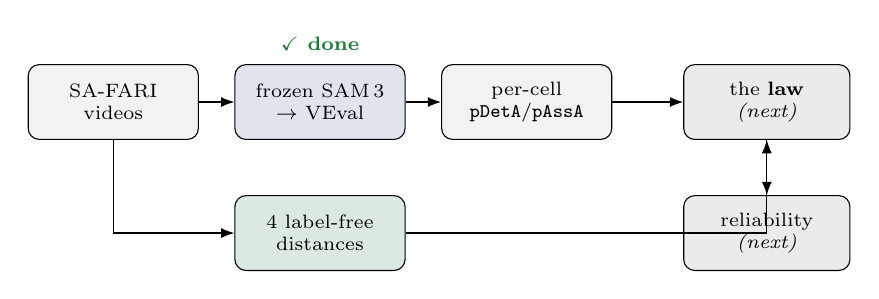
\begin{tikzpicture}[>=Latex,
    box/.style={draw,rounded corners,align=center,font=\scriptsize,inner sep=3pt,text width=1.95cm,minimum height=0.95cm}]
    \node[box,fill=black!5] (saf) {SA-FARI\\videos};
    \node[box,fill=navy!14,right=0.45cm of saf] (sam) {frozen SAM\,3\\$\to$ VEval};
    \node[box,fill=black!5,right=0.45cm of sam] (sco) {per-cell\\\texttt{pDetA}/\texttt{pAssA}};
    \node[box,fill=forest!16,below=0.7cm of sam] (dist) {4 label-free\\distances};
    \node[box,fill=black!8,right=0.9cm of sco,text width=1.9cm] (law) {the \textbf{law}\\\itshape (next)};
    \node[box,fill=black!8,below=0.7cm of law,text width=1.9cm] (rel) {reliability\\\itshape (next)};
    \draw[->] (saf)--(sam); \draw[->] (sam)--(sco);
    \draw[->] (saf.south) |- (dist.west);
    \draw[->] (sco)--(law); \draw[->] (dist.east) -| (law.south);
    \draw[->] (law)--(rel);
    \node[forest,font=\scriptsize\bfseries,above=0.05cm of sam] {\ck\ done};
    \node[forest,font=\scriptsize\bfseries,left=0.05cm of dist] {};
  \end{tikzpicture}
  \vspace{0.5em}
  \begin{itemize}\footnotesize
    \item \done\ \textbf{Done \& validated:} the data pipeline, the four distances, and the frozen-SAM\,3
          measurement --- everything that produces the inputs $X$ and the outputs $Y$.
    \item \textcolor{burnt}{\textbf{Next:}} fit the small \emph{law} $X\!\to\!Y$ and turn it into a
          reliability estimate (this talk stops before it).
  \end{itemize}
\end{frame}

% ------------------------------------------------------------ distances
\begin{frame}{The four ``how new is it?'' distances \small(all built, sanity-checked)}
  \begin{itemize}
    \item \textbf{Taxonomic} --- steps up the tree of life to the nearest known species.
    \item \textbf{Visual} --- cut the animal out of the frame, ``fingerprint'' it (DINOv2), compare to
          known species.
    \item \textbf{Environment} --- \emph{erase} the animal, fingerprint the leftover scene, compare to
          known places; plus a \textbf{night/infrared} flag.
    \item \textbf{Temporal} --- how many years to the nearest known footage.
  \end{itemize}
  \vspace{0.3em}
  \begin{block}{The one rule that keeps it honest}
    \centering\footnotesize Every distance is computed against the \frozen{reference (``seen'') set only}
    --- no information about the target animal can leak in. A test proves a species can never fake
    ``distance 0'' to itself.
  \end{block}
\end{frame}

% ------------------------------------------------------------ measuring SAM 3
\begin{frame}{Measuring SAM\,3 --- the numbers we predict}
  \centering
  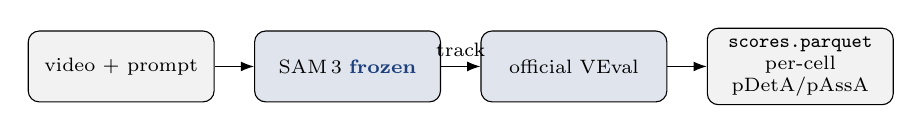
\begin{tikzpicture}[>=Latex,
    box/.style={draw,rounded corners,align=center,font=\scriptsize,inner sep=3pt,text width=2.15cm,minimum height=0.9cm}]
    \node[box,fill=black!5] (t) {video $+$ prompt};
    \node[box,fill=navy!14,right=0.5cm of t] (sam) {SAM\,3 \frozen{frozen}};
    \node[box,fill=navy!14,right=0.5cm of sam] (ve) {official VEval};
    \node[box,fill=black!5,right=0.5cm of ve] (sc) {\texttt{scores.parquet}\\per-cell pDetA/pAssA};
    \draw[->] (t)--(sam); \draw[->] (sam)--node[midway,above,font=\scriptsize]{track}(ve); \draw[->] (ve)--(sc);
  \end{tikzpicture}
  \vspace{0.5em}
  \begin{itemize}\footnotesize
    \item Our harness runs frozen SAM\,3 over \textbf{every clip} and the \textbf{official} scorer turns
          its outlines into detection/association numbers --- one row per \textbf{(species, place, year)} cell.
    \item Built to be \textbf{resumable} (a Colab timeout never loses progress); the full test split ran on
          one A100 in $\sim$3\,hours.
  \end{itemize}
\end{frame}

% ------------------------------------------------------------ GATE 1 results
\begin{frame}{Gate\,1 --- the measurement is validated}
  \begin{columns}[T]
    \begin{column}{0.44\textwidth}
      \centering
      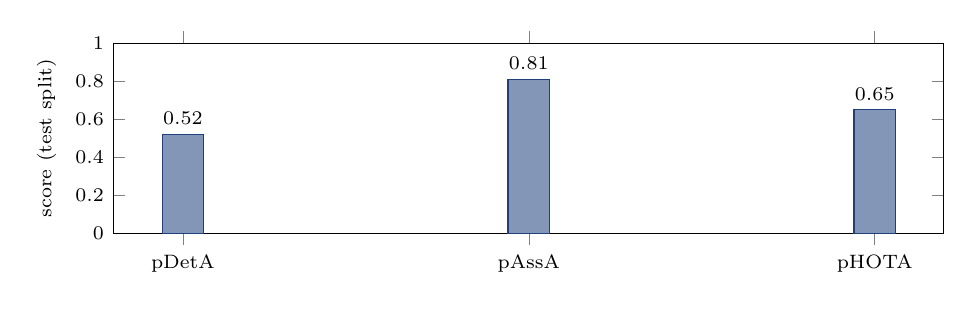
\begin{tikzpicture}
      \begin{axis}[width=\textwidth,height=4.0cm,ybar,bar width=15pt,
        symbolic x coords={pDetA,pAssA,pHOTA},xtick=data,
        ylabel={\scriptsize score (test split)},ymin=0,ymax=1,nodes near coords,
        every node near coord/.append style={font=\scriptsize},
        tick label style={font=\scriptsize},label style={font=\scriptsize}]
      \addplot[fill=navy!55,draw=navy] coordinates {(pDetA,0.52)(pAssA,0.81)(pHOTA,0.65)};
      \end{axis}
      \end{tikzpicture}\\[-2pt]
      {\scriptsize zero-shot SAM\,3, full test split}
    \end{column}
    \begin{column}{0.54\textwidth}
      \footnotesize Three independent checks say the numbers are right:
      \begin{itemize}\footnotesize
        \item \ck\ \textbf{Internally consistent:} $\text{pHOTA}\approx\sqrt{\text{pDetA}\cdot\text{pAssA}}
              =\sqrt{0.52\cdot0.81}=0.65$.
        \item \ck\ \textbf{Matches the paper:} our zero-shot $0.65 + $ the paper's $+0.196$ fine-tuning gain
              $\approx 0.84$ $=$ their \emph{fine-tuned} SAM\,3.
        \item \ck\ \textbf{Clean on hard negatives:} SAM\,3 essentially \textbf{never invents} an animal
              that isn't there.
      \end{itemize}
    \end{column}
  \end{columns}
  \vspace{0.2em}
  \centering\footnotesize The whole measurement pipeline reproduces published SAM\,3 performance end-to-end.
\end{frame}

% ------------------------------------------------------------ what it shows
\begin{frame}{What the result already shows}
  \begin{columns}[T]
    \begin{column}{0.5\textwidth}
      \begin{itemize}\footnotesize
        \item \textbf{Finding and following are far apart} (\texttt{pDetA} $0.52$ vs \texttt{pAssA}
              $0.81$): SAM\,3 tracks well once it \emph{finds} an animal, but misses about half of them.
        \item Per species, \textbf{finding} spans almost the full range --- easy, distinctive animals high;
              small, cryptic ones low.
        \item \emph{That spread is the signal} a predictor can learn. If every species scored alike, there
              would be nothing to predict.
      \end{itemize}
    \end{column}
    \begin{column}{0.5\textwidth}
      \centering
      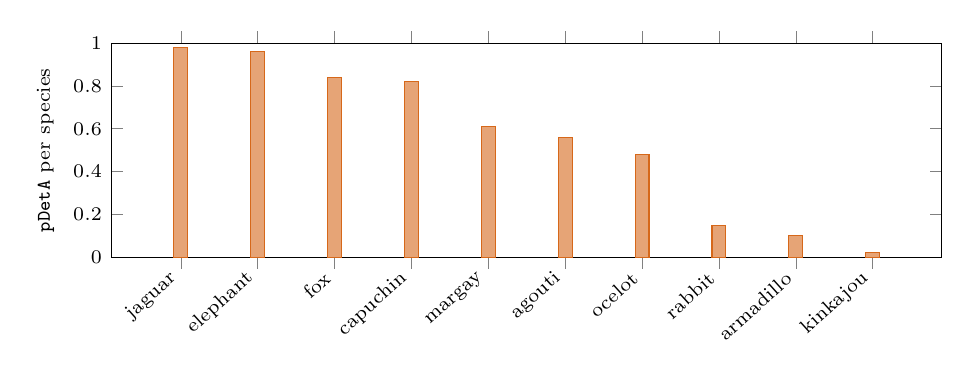
\begin{tikzpicture}
      \begin{axis}[width=\textwidth,height=4.3cm,ybar,bar width=5pt,
        symbolic x coords={jaguar,elephant,fox,capuchin,margay,agouti,ocelot,rabbit,armadillo,kinkajou},
        xtick=data,x tick label style={rotate=42,anchor=east,font=\scriptsize},
        ylabel={\scriptsize \texttt{pDetA} per species},ymin=0,ymax=1,
        tick label style={font=\scriptsize},label style={font=\scriptsize}]
      \addplot[fill=burnt!60,draw=burnt] coordinates
        {(jaguar,0.98)(elephant,0.96)(fox,0.84)(capuchin,0.82)(margay,0.61)(agouti,0.56)(ocelot,0.48)(rabbit,0.15)(armadillo,0.10)(kinkajou,0.02)};
      \end{axis}
      \end{tikzpicture}
    \end{column}
  \end{columns}
\end{frame}

% ------------------------------------------------------------ engineering
\begin{frame}{Built to be trusted}
  \begin{itemize}
    \item \textbf{Config-driven \& typed} --- an experiment changes a \emph{value}, never the code; a
          growing automated test suite guards every rule.
    \item \textbf{The leakage firewall} is enforced in code \emph{and} tested --- no test-set information
          can enter a distance, so a ``prediction'' can never be trivially right.
    \item \textbf{Reproducible on a borrowed GPU} --- resumable runs, parallelised downloads, and the
          \emph{official} evaluator (never re-implemented).
  \end{itemize}
  \vspace{0.3em}
  \begin{block}{}
    \centering\footnotesize Everything above is committed, tested, and reproduces the published SAM\,3
    numbers --- a solid foundation for the modelling half.
  \end{block}
\end{frame}

% ------------------------------------------------------------ next
\begin{frame}{Where we are, and what's next}
  \begin{block}{Done \& validated}
    \centering\footnotesize
    Data pipeline \ck\;\; four label-free distances \ck\;\; frozen-SAM\,3 measurement \ck\;\;
    \textbf{Gate\,1 passed} \ck
  \end{block}
  \vspace{0.5em}
  \begin{itemize}
    \item \textcolor{burnt}{\textbf{Next:}} fit a small \textbf{law} --- distance in $\to$ predicted
          \texttt{pDetA}/\texttt{pAssA} out --- and check it predicts \emph{held-out} species and places
          (Gate\,2: does out-of-sample signal really exist?).
    \item Then the deployment tool: a new (species, place) $\to$ a prediction $+$ a confidence interval.
  \end{itemize}
  \vspace{0.4em}
  \centering\small\color{navy}\textbf{Thank you --- questions welcome.}
\end{frame}

\end{document}
